\insertmeeting 
	{States Planning Party} 
	{01/31/23} 
	{Hagerty High School}
	{Karissa, Laura, Tyler, Mohana, Samantha, Jorge, Ritam, Nathan, Robert, Jensen}
	{Images/RobotPics/robot.jpg}
	{2:30 - 4:30}
	
\hhscommittee{General}
\noindent\hfil\rule{\textwidth}{.4pt}\hfil
\subsubsection*{Goals}
\begin{itemize}
    \item Use planning organizers to set little goals for each committee for future improvement
    \item Discuss robot and non-robot things that should be worked on

\end{itemize} 

\noindent\hfil\rule{\textwidth}{.4pt}\hfil

\subsubsection*{Accomplishments}
Today, we created a backwards plan for States, which is basically a method of planning that begins with establishing a clear end goal, and working backwards to figure out the steps the team must take in order to get there. Once we made some goals, we got straight to work. The software committee began their fine tuning of autonomous, where they tweaked Vision, and programmed the picking up and placement of cones onto the Leagues Lift. They also worked on improving cone detection with OpenCV in order to be able to pick them up more efficiently. The hardware committee began work on a new lift. They CADed the rollers and their panels for the poles, and started working on the servo plate in the center. Work on the lift will be stalled until the poles are placed on the drivetrain (also in CAD), where the plate will then be finished up. The technical writing committee started to adjust the Engineering Notebook, correcting some of the errors they noticed after it was printed for the Space Coast League Competition.


% \begin{figure}[ht]
%   \centering
%   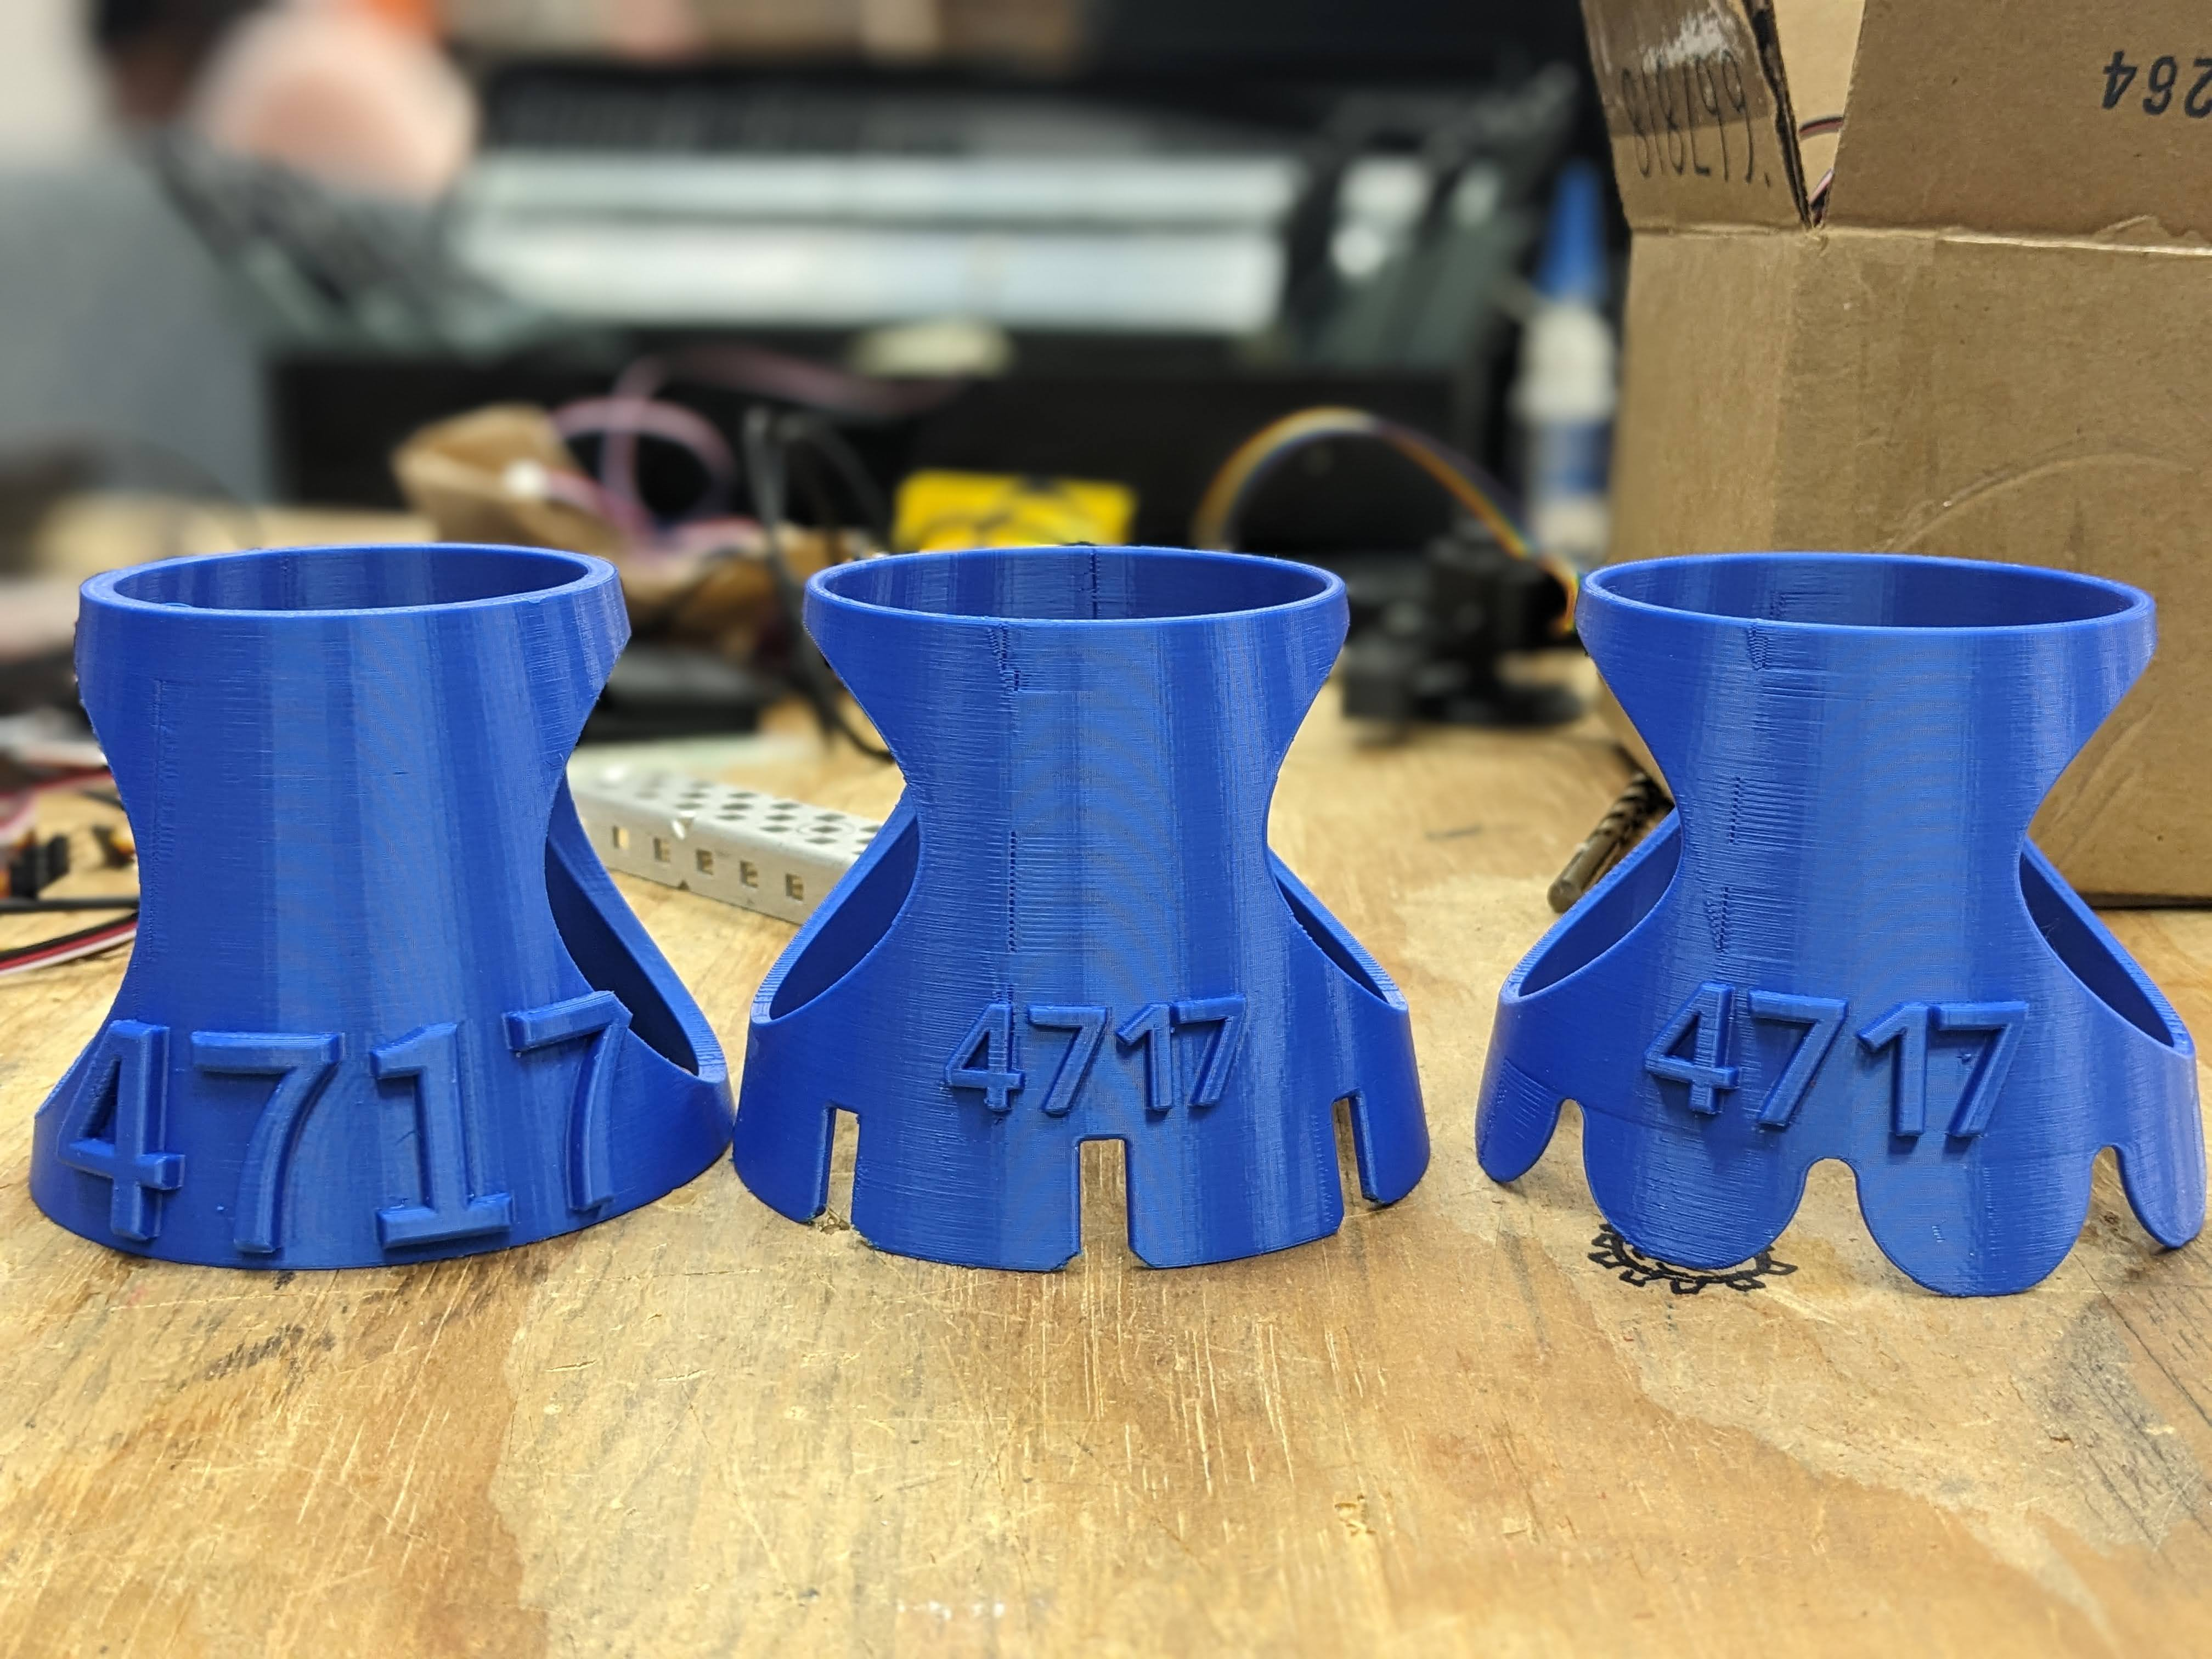
\includegraphics[width=0.95\textwidth]{Meetings/January/01-24-23/01-24-23-TElement.jpg}
%   \caption{Old to new variation of team beacon}
%   \label{fig:pic1}
% \end{minipage}
% \end{figure}

% \begin{figure}[ht]
%   \centering
%   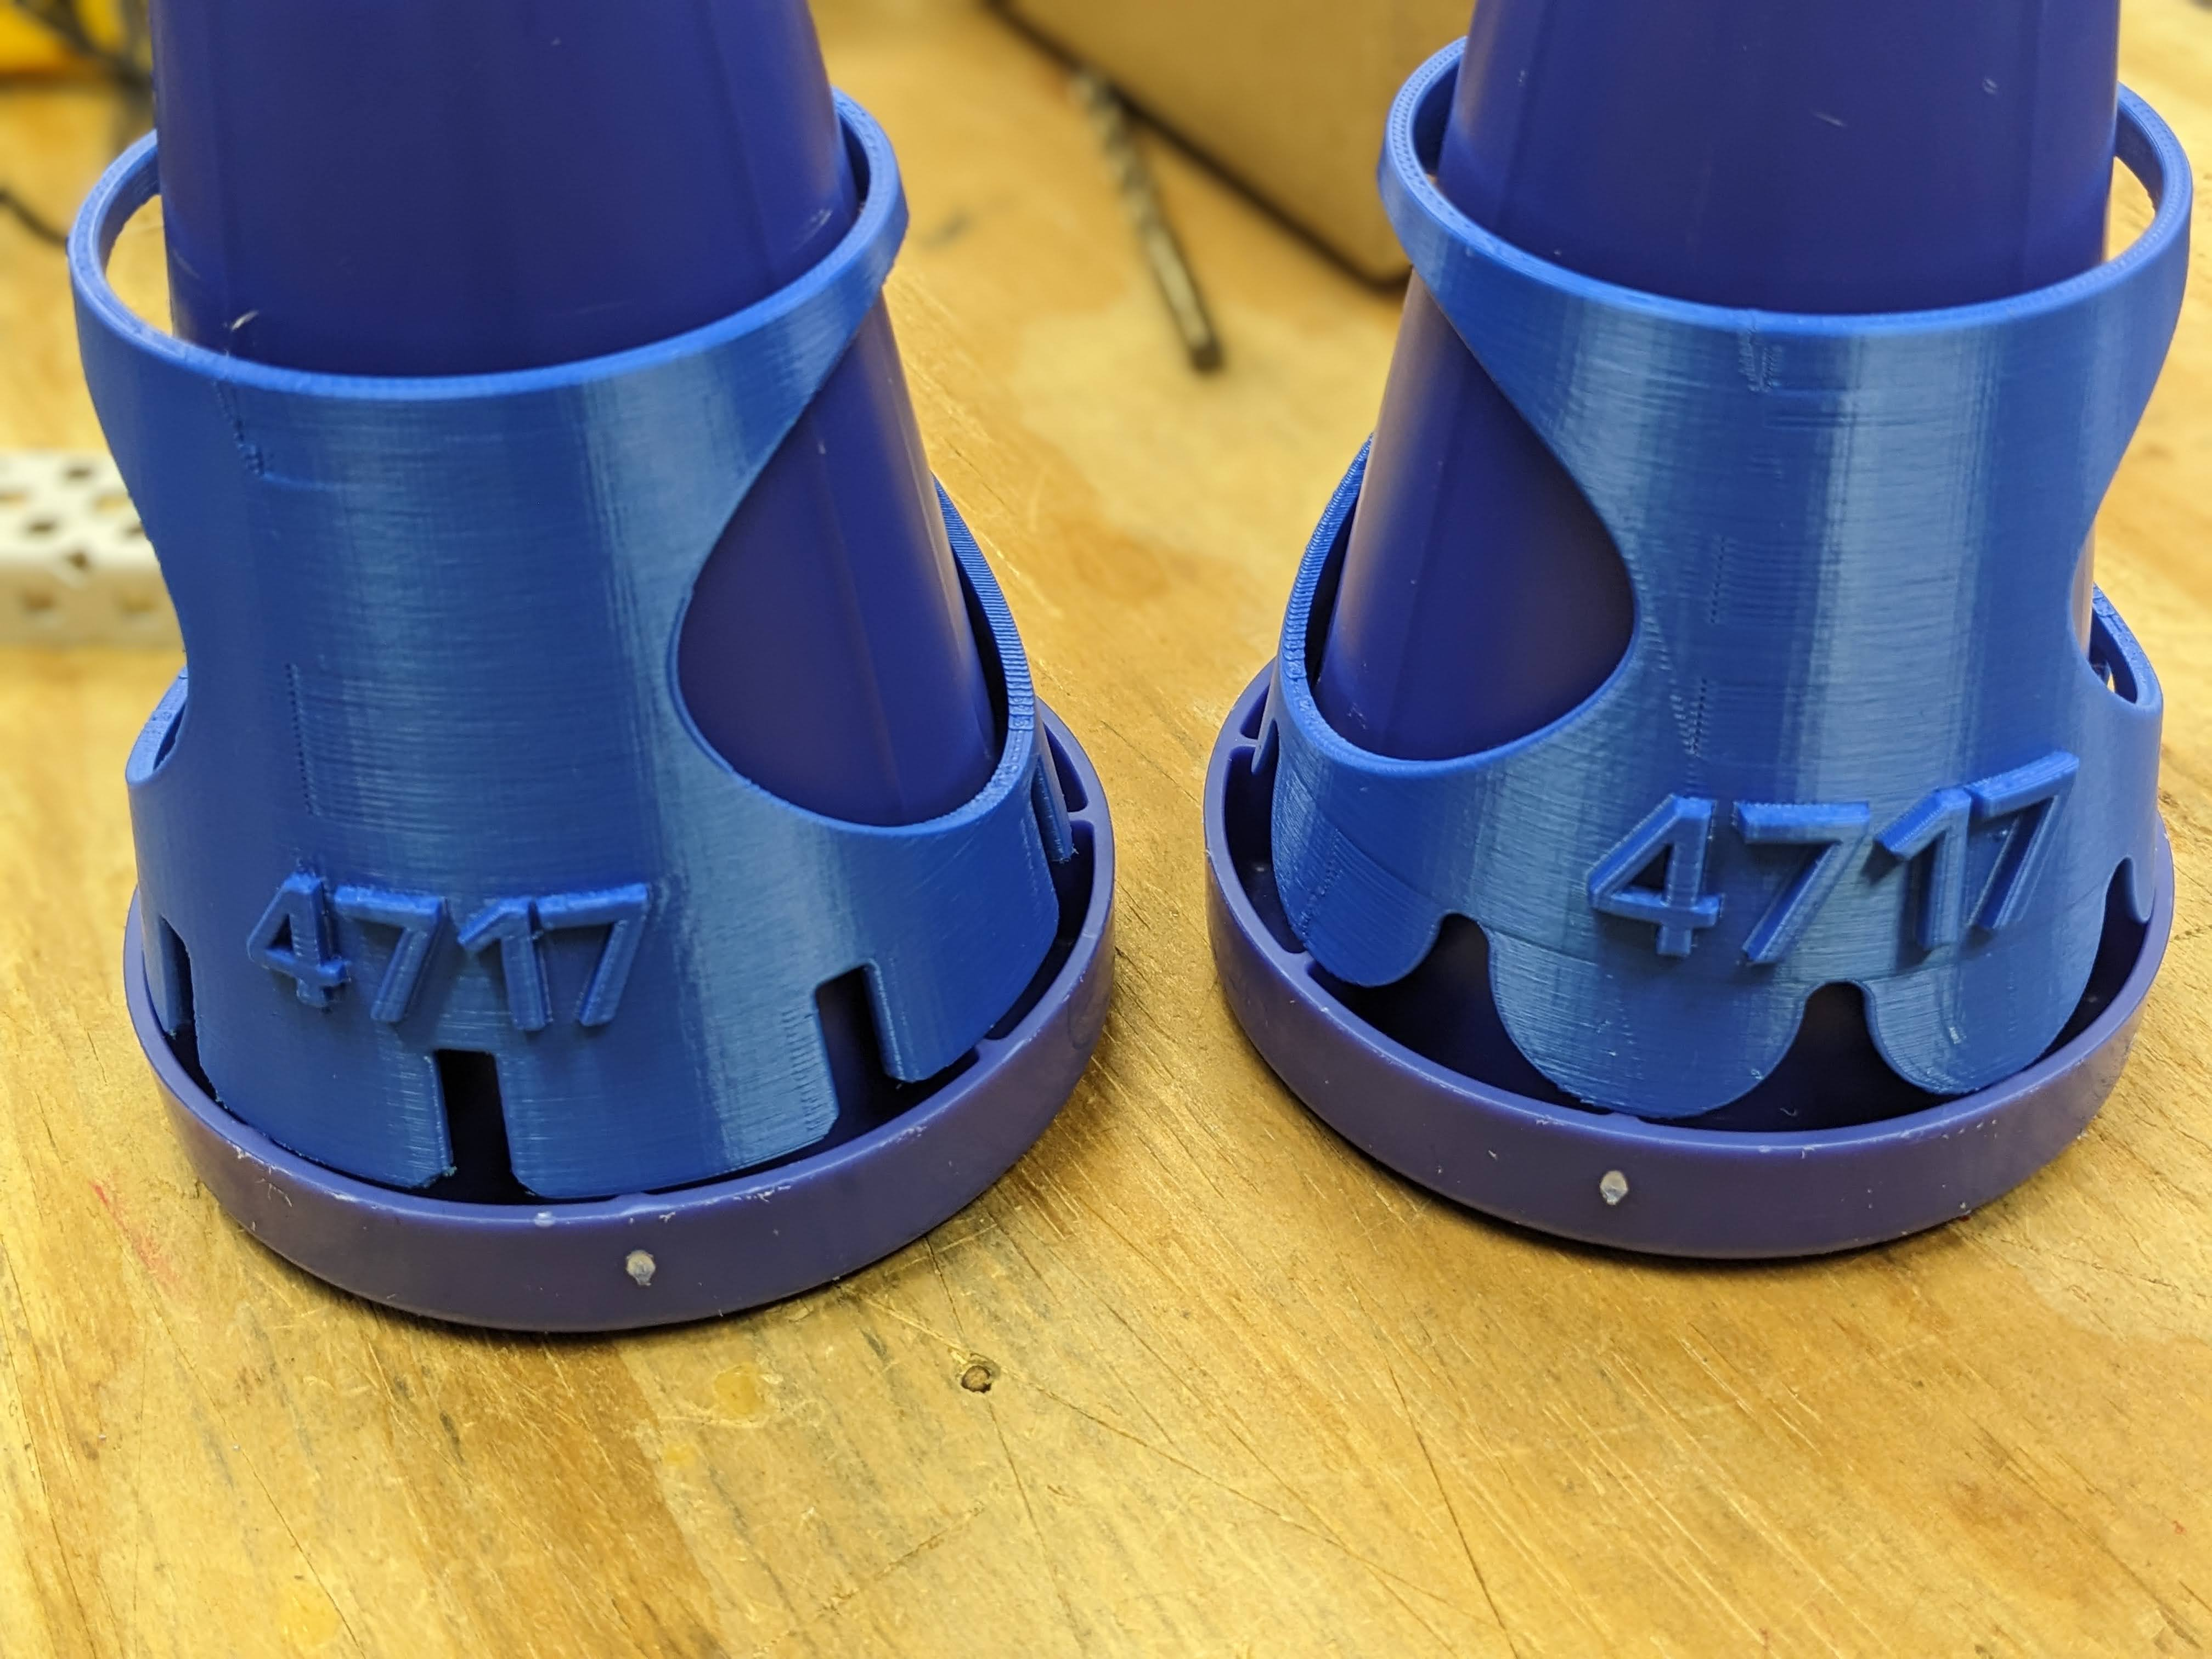
\includegraphics[width=0.95\textwidth]{Meetings/January/01-24-23/01-24-23-TElement2.jpg}
%   \caption{Beacon}
%   \label{How our new (right) team beacon fits on a cone}
% \end{minipage}
% \end{figure}


\whatsnext{
\begin{itemize}
    \item Start CADing new/improved parts
    \item Edit notebook, make sure everything is up to date
    \item Improve Promote video script
    \item Update Sponsor letters and brochures
\end{itemize} 
}
